\documentclass[a4paper,12pt]{article}

\usepackage[dutch]{babel}
\usepackage{fancyhdr}
\usepackage{graphicx}
\usepackage[pdftex,bookmarks=true]{hyperref}
\usepackage[utf8]{inputenc}
\usepackage{fullpage}
\usepackage{parskip}
\usepackage{float}
\usepackage{subcaption}

\title{Samenvatting Ontwerpen III \\ \large HoGent}
\author{Lorenz Verschingel}

\begin{document}
\maketitle
\section{Factory Pattern}
We pakken de code voor de creatie op en verplaatsen deze naar een ander object dat alleen maar het maken van producten als taak zal hebben.
Dit object noemen we \textit{Factory}.

\subsection{Simple Factory}
\begin{figure}[H]
\centering
  	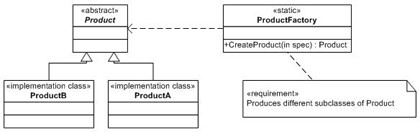
\includegraphics[width=.5\linewidth]{img/Factory/SimpleFactory.jpg}
  	\caption{UML: Simple Factory}
  	\label{fig:SimpleFactory}
\end{figure}

Volgens de UML in figuur~\ref{fig:SimpleFactory} kan de ProductFactory producten van het type Product afleveren aan zijn cliënten.

\subsection{Factory Methode}
\begin{figure}[H]
\centering
  	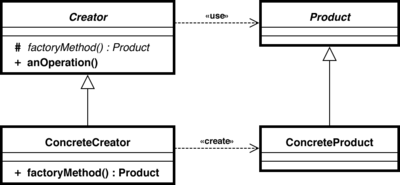
\includegraphics[width=.5\linewidth]{img/Factory/FactoryMethod.png}
  	\caption{UML: Factory Methode}
  	\label{fig:FactoryMethod}
\end{figure}

Ten opzichte van figuur~\ref{fig:SimpleFactory} is er niet zoveel veranderd.
In figuur~\ref{fig:FactoryMethod} is de Factory klasse abstract geworden en is de create methode ook abstract.
Deze wordt dan later door een concrete factory geïmplementeerd.

Het Factory Method Pattern definieert een interface voor het creëren van een object, maar laat de subklassen beslissen welke klasse er geïnstantieerd wordt.
De Factory Method draagt de instanties over aan de subklassen.

\subsection{Dependency Inversion-principe}
Wees afhankelijk van abstracties, niet afhankelijk van concrete klassen.

\subsection{Abstract Factory Pattern}
\begin{figure}[H]
\centering
  	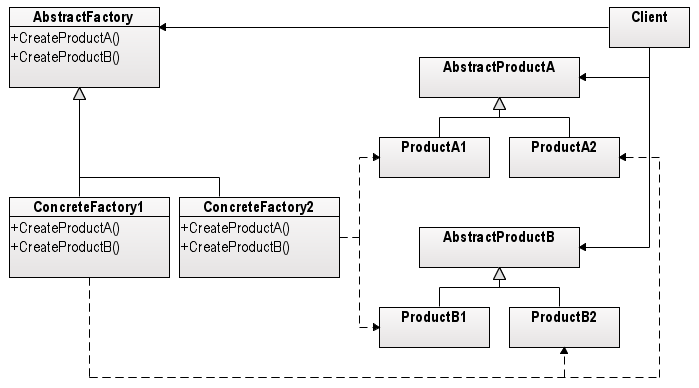
\includegraphics[width=.7\linewidth]{img/Factory/AbstractFactory.png}
  	\caption{UML: Abstract Factory}
  	\label{fig:AbstractFactory}
\end{figure}

Het Abstract Factory Pattern levert een interface voor de vervaardiging van reeksen gerelateerde of afhankelijke objecten zonder hun concrete klassen te specificeren.

\section{Iterator Pattern}
\begin{figure}[H]
\centering
  	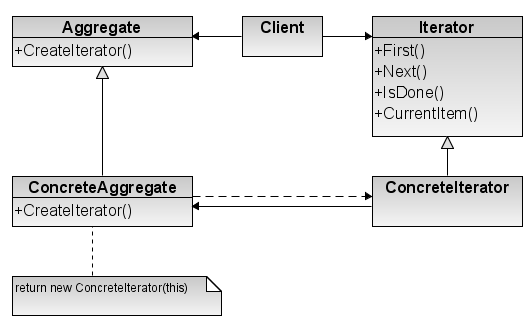
\includegraphics[width=.7\linewidth]{img/Iterator.png}
  	\caption{UML: Iterator Pattern}
  	\label{fig:Iterator}
\end{figure}

Het Iterator Pattern voorziet ons van een manier voor sequentiële toegang tot de elementen van een aggregaatobject zonder de onderliggende representatie weer te geven.

Figuur~\ref{fig:Iterator} heeft een redelijk uitgebreide verantwoordelijkheid aan de iterator. In de meeste gevallen volstaat het om een methode hasNext() en Next() in te voeren.

Java voorziet het iterator pattern met de klasse Iterator.
Hiervoor moet men zorgen dat de iterator-klasse de klasse Iterator van Java gebruikt en dat de methode createIterator() het type Iterator$<$teItererenType$>$ terug geeft.

\section{Composite Pattern}
Het Composite Pattern stelt je in staat om objecten in boomstructuren samen te stellen om partwhole hiërarchiën weer te geven.
Composite laat clients de afzonderlijke objecten of samengestelde objecten op uniforme wijze behandelen.

Beschouw figuur~\ref{fig:Composite}.
De klasse Component is een interface voor alle objecten in de compositie.
Een leaf definiëert het gedrag voor de elementen in de compositie.
Dit gebeurt via implementatie van de operaties die de klasse Composite ondersteunt.
De klasse Composite definiëert het gedrag van de component met kinderen. Deze klasse moet ook alle kinderen kunnen bijhouden.

Zowel Composite als Leaf overriden enkel de methoden die zin hebben, en gebruiken de standaardimplementatie uit Component voor de methoden die niet zinnig zijn.

\begin{figure}[H]
\centering
  	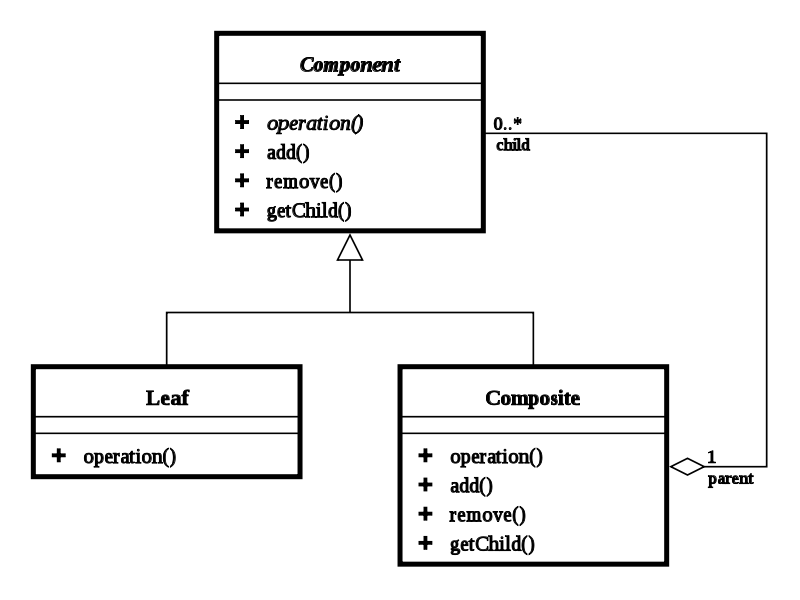
\includegraphics[width=.7\linewidth]{img/Composite.png}
  	\caption{UML: Composite Pattern}
  	\label{fig:Composite}
\end{figure}

\subsection{De compositie-iterator}
Om een Composite-iterator te implementeren voegen we de methode createIterator() toe aan iedere component.
Voor de Composite klasse geeft deze methode een iterator over zijn kinderen terug, voor de klasse Leaf een NullIterator. Als over de hele boomstructuur geïtereerd moet worden dan moet de iterator van de root in een CompositeIterator klasse verpakt worden.

De klasse CompositeIterator implementeert de interface Iterator.
Verder bevat deze klasse een stack waarop alle afzonderlijke Iterators geplaatst kunnen worden.

\section{Command Pattern}
Het Command Pattern schermt een aanroep af door middel van een object, waarbij je verschillende aanroepen in verschillende objecten kan opbergen, in een queue kan zetten of op schijf kan bewaren.
Vaak worden ook undo-operaties ondersteund.

Het command pattern wordt gebruikt om een actie voor te stellen als een object. De commands bevatten alle info die ze nodig hebben om de actie te kunnen uitvoeren. Nieuwe commando's kunnen eenvoudig worden toegevoegd.

In figuur~\ref{fig:Command} zorgt de Client ervoor dat de Invoker het juiste commando kent. Later kan de Client dan ook aan de Invoker vragen om het commando uit te voeren.

\begin{figure}[H]
\centering
  	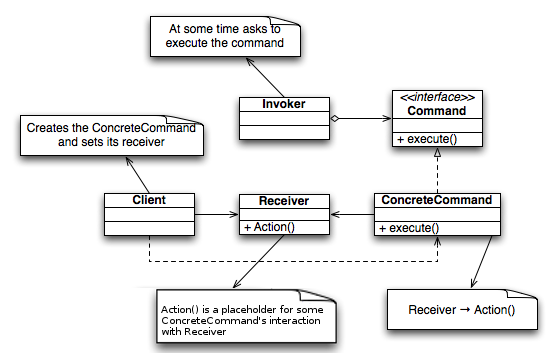
\includegraphics[width=.7\linewidth]{img/CommandPattern.png}
  	\caption{UML: Command Pattern}
  	\label{fig:Command}
\end{figure}

\subsection{Macro-Command}
Een macro-command houdt een lijst bij met allerlei commando's.
Bij het uitvoeren van het macro-commando voert deze dan alle commando's die in de lijst zitten één voor één uit.

\subsection{Toepassingen}
\begin{itemize}
\item Aanvragen in een wachtrij
\item Logging aanvragen
\item ASP.NET MVC: Klasse ActionResult met methode ExecuteResult().
\end{itemize}

\section{Template Method Pattern}
Het Template Method Pattern definieert het skelet van een algoritme in een methode, waarbij sommige stappen aan subklassen worden overgelaten.
De Template method laat subklassen bepaalde stappen in een algoritme herdefiniëren zonder de structuur van het algoritme te veranderen.

\begin{figure}[H]
\centering
  	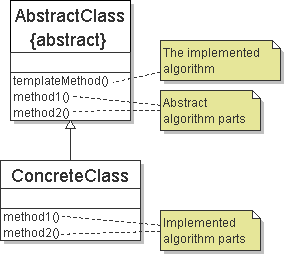
\includegraphics[width=.5\linewidth]{img/Template/Template.png}
  	\caption{UML: Template Pattern}
  	\label{fig:Template}
\end{figure}

\subsection{Inhaken in een Template Method}
In de template method kan men een conditionele opdracht toevoegen. Deze methode heeft een (bijna) lege standaard implementatie. Deze methode noemt men dan de hook. Een subklasse kan deze methode overriden maar dit is niet verplicht.

\begin{figure}[H]
\centering
  	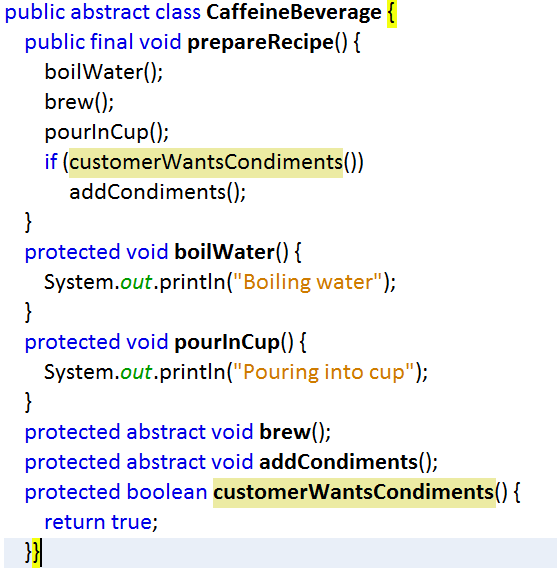
\includegraphics[width=.5\linewidth]{img/Template/VoorbeeldHook.png}
  	\caption{Code met hook}
  	\label{fig:VoorbeeldHook}
\end{figure}

In figuur~\ref{fig:VoorbeeldHook} is de methode customerWantCondiments() de hook. Enkel als deze methode waar is dan wordt de methode addCondiments() opgeroepen.

\section{Builder Pattern}
Gebruik het Builder pattern om de constructie van een product af te schermen en zorg dat je het in stappen kan construeren.

Mogelijke hints hiervoor zijn:
\begin{itemize}
\item Constructor met veel parameters
\item Klasse met veel constructors
\item Samengesteld object
\end{itemize}

\begin{figure}[H]
\centering
  	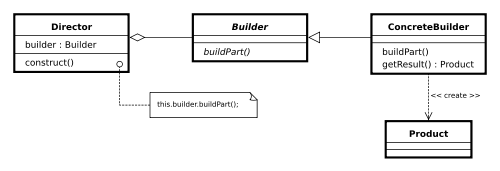
\includegraphics[width=.7\linewidth]{img/Builder/Builder.png}
  	\caption{UML: Builder pattern}
  	\label{fig:Builder}
\end{figure}

In figuur~\ref{fig:Builder} is de klasse Builder een abstracte interface voor de creatie van de onderdelen van het Product object.
De ConcreteBuilder bouwt de onderdelen van het complexe object en gooit deze samen door implementatie van de Builder interface.
Het houdt een representatie van het object bij en biedt een interface voor het opvragen van het product.
De Director klasse bouwt het complexe object gebruik makend van de interface van de Builder.

De voordelen van het Builder Pattern zijn dat de manier waarop een complex object gebouwd wordt afgeschermt is.
Het geeft ook de mogelijkheid om objecten in meerdere stappen en wisselende processen te maken.
(Dit in tegenstelling tot Factory Pattern.)
Het verbergt de interne representatie van het product voor de client.
En tot slot kunnen Productimplementaties steeds wisselen, dit is zo omdat de client alleen een abstracte interface ziet.

Een nadeel van het Builder Pattern is dat het maken van een object meer domeinkennis vereist van de client dan bij het Factory Pattern. Dit kan opgelost worden door een Director klasse toe te voegen.

\subsection{Variant}
Deze variant is bedoeld voor de constructie van klasses met
\begin{itemize}
\item veel opties.
\item veel argumenten bij constructie.
\item mogelijks ook al veel default waarden.
\end{itemize}
Men kan dan de Builder klasse als een interne klasse implementeren.

\begin{figure}[H]
\centering
  	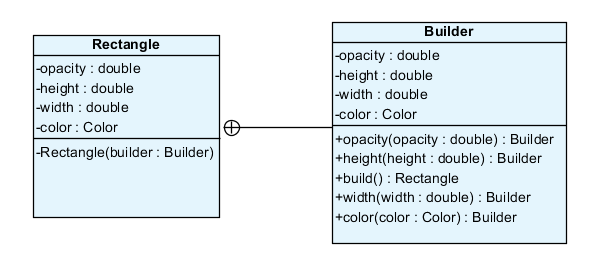
\includegraphics[width=.7\linewidth]{img/Builder/BuilderVariant.png}
  	\caption{Voorbeeld: Variant van het Builder Pattern}
  	\label{fig:BuilderVariant}
\end{figure}

Als de code bij figuur~\ref{fig:BuilderVariant} geïmplementeerd wordt dan wordt bij de constructie van de rechthoek alle attributen uit de builder opgehaald.
Constructie van de rechthoek gebeurt daar de static Builder aan te spreken en zo alle attributen mee te geven.
Nadat alle atributen zijn gemaakt kan met met behulp van de static Builder de rechthoek construeren.

Merk ook op dat de meeste "setters" van de klasse Builder ook een Builder retourneren. Dit is dan het eigenlijke Builder-object waarop iets werd toegevoegd.

\section{Singleton}
Een singleton is een uniek object waarvoor er slechts één instantie bestaat.
Indien er meerdere instanties van dit object zouden zijn, resulteert dit gegarandeerd in problemen.
Het singleton garandeert dan ook dat er maar één en niet meer dan één instatie van een bepaalde klasse bestaat.
Verder levert de klasse één globaal toegangspunt.
De instatie van de klasse wordt pas aangemaakt op het moment dat dit nodig is (=Lazy Loading).

In het kort:

Het Singleton Pattern garandeert dat een klasse slechts één
instantie heeft, en biedt een globaal toegangspunt ernaartoe.

\begin{figure}[H]
\centering
  	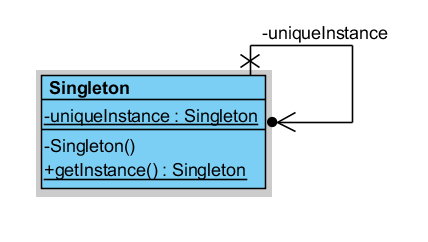
\includegraphics[width=.7\linewidth]{img/Singleton/Singleton.png}
  	\caption{UML: Singleton}
  	\label{fig:Singleton}
\end{figure}

In figuur~\ref{fig:Singleton} ziet men dat het Singleton een uniek object van het type Singleton bijhoudt. Omdat dit Singleton altijd hetzelfde object moet zijn is dit attribuut static. Om dezelfde reden is de methode getInstance() ook static.

\subsection{Problemen bij multithreading}
Als er niet ingegrepen wordt kunnen er toch meerdere instanties van het Singleton object bestaan.
Dit kan tot ernstige problemen leiden.
Toch kan dit probleem relatief makkelijk opgelost worden in Java.

Een eerste oplossing is zonder lazy loading. Men zorgt dat het Singleton-object final is en er wordt ook meteen een instantie gemaakt. Hiervoor kan de code uit figuur~\ref{fig:SingletonEagerLoading} bekeken worden.

Een tweede oplossing is om de static methode getInstance synchronised te maken. Zo kan men weer gebruik maken van lazy loading, maar men dient wel te besteffen dat synchronisatie duur is. Het kan de performatie met een factor 100 reduceren. Ook is de synchronisatie overbodig nadat de code voor de eerste maal is doorlopen. De code hiervoor kan in figuur~\ref{fig:SingletonLazyLoading} bezichtigd worden.

\begin{figure}[H]
\centering
\begin{subfigure}{.49\textwidth}
  \centering
  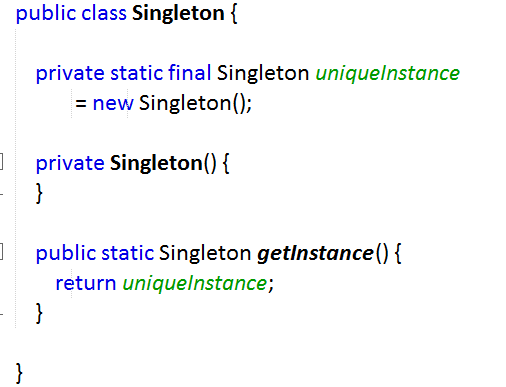
\includegraphics[width=.9\linewidth]{img/Singleton/SingletonZonderLazyLoading.png}
  \caption{Singleton met Eager Loading}
  \label{fig:SingletonEagerLoading}
\end{subfigure}
\begin{subfigure}{.49\textwidth}
  \centering
  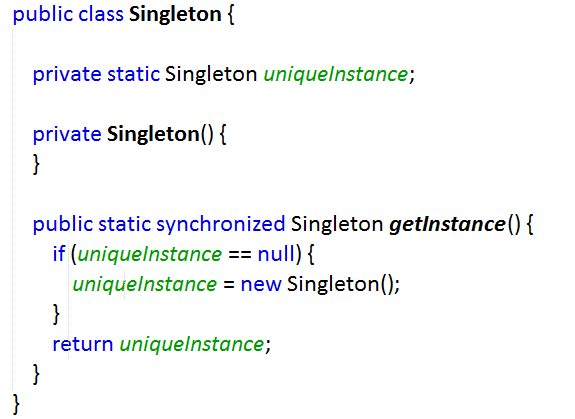
\includegraphics[width=.9\linewidth]{img/Singleton/SingletonMetLazyLoading.png}
  \caption{Singleton met Lazy Loading}
  \label{fig:SingletonLazyLoading}
  \end{subfigure}
\caption{Code: multithreading safe}
\label{fig:SingletonMultithreadSafe}
\end{figure}

\end{document}